\documentclass{article}
\usepackage[utf8]{inputenc}
\usepackage[english, russian]{babel}
\usepackage[margin=3cm]{geometry}
\usepackage{paralist}
\usepackage{amsthm, amsmath, amsfonts, amssymb}
\usepackage{mathtools} % \mathclap
\usepackage{bm}
\usepackage{dsfont}
\usepackage{hyperref}
\usepackage{tabularx}
\usepackage{graphicx}
\usepackage{multirow}
\usepackage{comment}
\usepackage{xcolor, colortbl}
\usepackage{xifthen, xspace}
\usepackage{caption, subcaption}
\usepackage{lscape}


\usepackage{sectsty}

\DeclareGraphicsExtensions{.png}

\setlength{\parindent}{10ex}


\title{Практическая работа №1.
    
Метод максимина, $\alpha-\beta$ отсечения, 
антогонистическая игра двух игроков в матричной форме

Вариант подготовлен для Новиков Данила Александрович}

\begin{document}

\maketitle

\section{Введение}

В рамках данной работы предстоит выполнить три задания. Все задания должны быть оформлены в электронном виде. 
Вам могут в этом помочь Word и редактор \href{https://inkscape.org/ }{Inkscape} либо любой другой векторный 
(типа Adobe Illustrator). \\\\
Файлы для заданий 1 и 2 отдельно выложены в векторном формате (svg) и в формате graphviz. \\
Решение необходимо оформить в файле формата PDF и отправить в Moodle. \\
Ссылка для отправки задания: \href{https://ivliyevsa-courses.mpei.ru/mod/assign/view.php?id=200}{https://ivliyevsa-courses.mpei.ru/mod/assign/view.php?id=200}\\\\
Структура титульного листа:
\begin{itemize}
\item название ВУЗа (Федеральное государственное бюджетное образовательное учреждение высшего 
профессионального образования «Национальный исследовательский университет «МЭИ»);
\item название кафедры (той, на которой вы учитесь);
\item название курса (Теория приниятия решений);
\item название работы (Практическая работа №1. Метод максимина, $\alpha-\beta$ отсечения, 
\item антагонистическая игра двух игроков в матричной форме);
\item имя-фамилия студента, группа;
\item имя-фамилия принимающего работу преподавателя (к.т.н., ст. преп. Ивлиев С.А.);
\item город (Москва) и год (2021).
\end{itemize}

\section{Задание №1}

Требуется рассчитать выигрыш игрока $A$ методом максимина. \\
Игроки ходят по очереди, сперва игрок $A$, 
потом игрок $B$, в листьях дерева проставлены выигришы игрока $A$.\\
К заданию прилагается дерево поиска в удобных для редактирования форматах svg (Inkscape, Adobe Illustrator) 
и gv (graphviz). \\
Ответом к заданию является заполненное дерево поиска. \\
Дерево поиска находится в приложении №1.

\section{Задание №2}

Требуется рассчитать выигрышь игрока $A$ используя метод $\alpha-\beta$ отсечения. \\
Игроки ходят по очереди, сперва игрок $A$, потом игрок $B$, в листьях дерева проставлены выигришы игрока $A$.\\
К заданию прилагается дерево поиска в удобных для редактирования форматах svg (Inkscape, Adobe Illustrator) и 
gv (graphviz). \\
Ответом к заданию является заполненное дерево поиска. Просмотренные вершины должны быть отмечены зелёным, 
отсечённые серым, линии к ним должны быть пунктирные. \\
Дерево поиска находится в приложении №1.

\section{Задание №3}

Требуется упростить матрицы игры и найти для неё седловую точку или показать, что её нет.\\
Ответом на задание является упрощённая матрица игры, с подсчитанной нижней и верхней границей игры и
седловой точкой, если она есть.

$$\begin{pmatrix}
5 &7 &2 &9 &2 &5 &5 &3 &8\\
7 &3 &2 &8 &4 &4 &5 &3 &8\\
8 &9 &6 &9 &8 &7 &10 &7 &10\\
5 &6 &2 &7 &3 &1 &8 &2 &5\\
5 &1 &5 &2 &8 &7 &9 &4 &7\\
7 &5 &3 &6 &5 &6 &9 &7 &8\\
7 &6 &5 &8 &4 &3 &7 &1 &9\\

\end{pmatrix}$$

\section{Литература}

Материалы к курсу доступны в системе Moodle: \href{https://ivliyevsa-courses.mpei.ru/course/view.php?id=13
}{https://ivliyevsa-courses.mpei.ru/course/view.php?id=13}

\begin{landscape}
    \section{Приложение №1}

    Дерево поиска для заданий 1 и 2.

    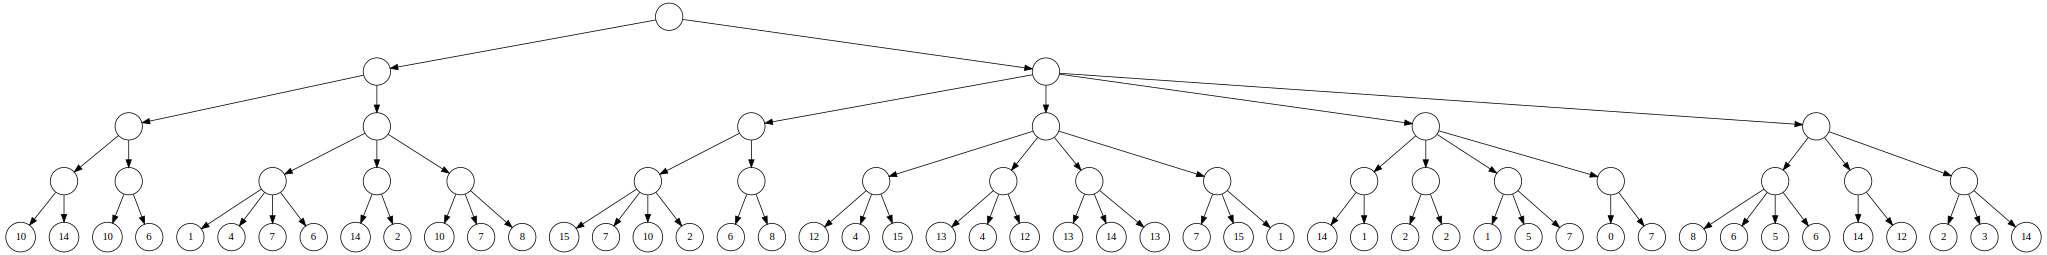
\includegraphics[width=200mm]{tree.png}
\end{landscape}




\end{document}